\begin{frame}
    \frametitle{Stage I-4: FHR Benchmark Phase III Goals}
    \begin{itemize}
        \item FHR Benchmark Phase III: 3D full core with feedback and multicycle 
        analysis
        \item I will use the open-source MSR simulation tool, Moltres, to conduct
        AHTR multiphysics simulations for fuel slab geometry and one-third 
        fuel assembly geometry. 
        \item Moltres, an application built atop the 
        \gls{MOOSE} parallel finite element framework \cite{gaston_moose:_2009}, 
        contains physics kernels and boundary conditions to solve arbitrary-group 
        deterministic neutron diffusion and thermal-hydraulics \glspl{PDE} 
        simultaneously on a single mesh \cite{lindsay_introduction_2018,park_advancement_2020}. 
        \item AHTR Moltres simulations will capture thermal feedback effects, 
        absent from the purely neutronics OpenMC simulations.  
    \end{itemize}
\end{frame}

\begin{frame}
    \frametitle{Stage I-4: FHR Benchmark Phase III Preliminary Work}
    \begin{itemize}
        \item To run Moltres simulations, the user provides group constant data from a neutron 
        transport solver, such as OpenMC, for the Moltres multigroup neutron diffusion 
        calculations and a mesh file representing the reactor geometry. 
        A TRISO-level fidelity mesh file is impractical and will result in an extremely 
        long Moltres runtime. 
        \item For successful AHTR Moltres simulation, I must establish 
        suitable spatial and energy homogenization that preserves accuracy while 
        maintaining an acceptable runtime.
    \end{itemize}
\begin{block}{Spatial Homogenization}
    \begin{itemize}
        \item I discretized the fuel slab into 13 cells: FLiBe, left graphite, right graphite, 
    and ten fuel cells (each cell has a different packing fraction)
    \end{itemize}
    \vspace{-0.3cm}
    \begin{figure}[]
        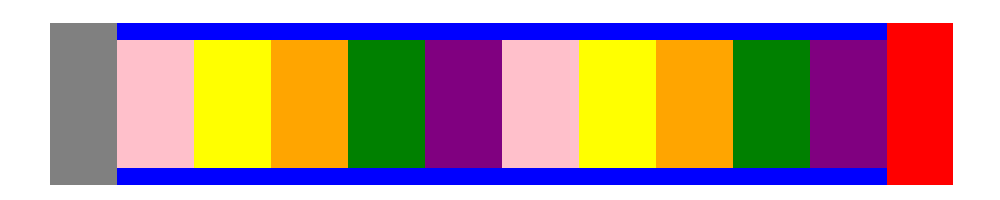
\includegraphics[width=0.7\linewidth]{../docs/figures/straightened_slab_mg.png}
        \caption{Straightened AHTR fuel slab spatially discretized into 
        13 \textit{cells} for OpenMC multigroup calculation.}
    \end{figure}
\end{block}
\end{frame}

\begin{frame}
    \frametitle{Stage I-4: FHR Benchmark Phase III Preliminary Work}
    \begin{block}{Energy Homogenization}
        \begin{itemize}
            \item I used the four group energy structure derived by Gentry et al. 
            \cite{gentry_development_2016} for AHTR geometries. 
        \end{itemize}
        \vspace{-0.4cm}
        \begin{table}[]
            \centering
            \begin{minipage}[c]{0.5\textwidth}
                \centering
                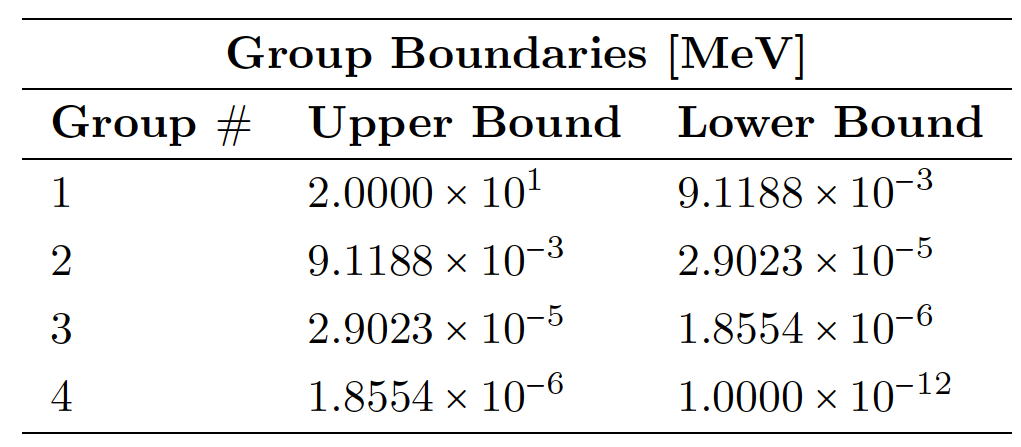
\includegraphics[width=0.6\linewidth]{figures/ahtr-energy-discr.png}
            \end{minipage}\hfill
            \begin{minipage}[c]{0.5\textwidth}
            \caption{4-group energy structures for AHTR geometry 
            derived by \cite{gentry_development_2016}.}
        \end{minipage}
        \end{table}
    \end{block}
    \vspace{-0.3cm}
    \begin{block}{Simulation Comparison: Continuous energy vs spatial 
        and energy homogenized}
        \begin{itemize}
            \item The 26pcm difference between $k_{eff}$ values is within both uncertainty values, 
            assuring that the spatial and energy homogenization used is suitable for generating 
            group constants for Moltres. 
        \end{itemize}
        \vspace{-0.3cm}
        \begin{table}[]
            \centering
            \begin{minipage}[c]{0.6\textwidth}
                \centering
                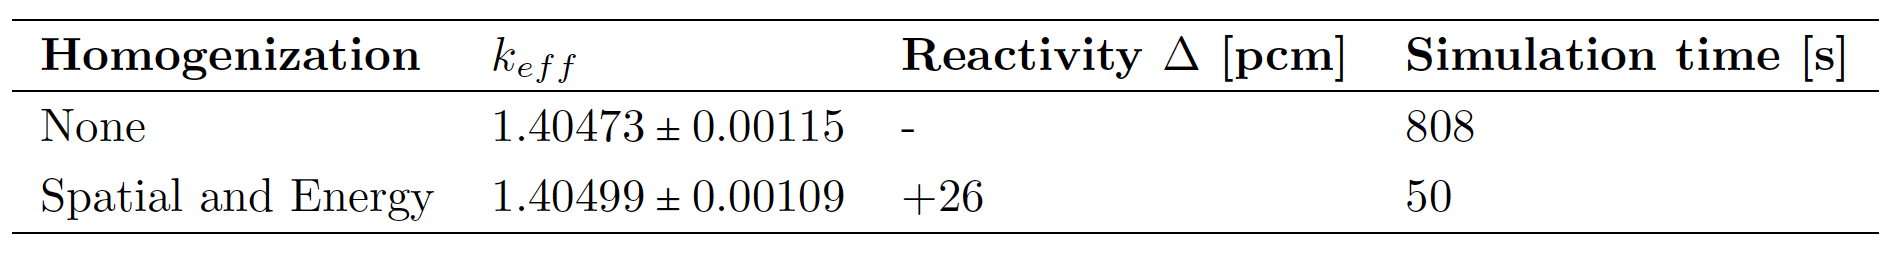
\includegraphics[width=0.8\linewidth]{figures/ahtr-homogenization.png}
            \end{minipage}\hfill
            \begin{minipage}[c]{0.4\textwidth}
            \caption{
            Both simulations were run on one BlueWaters XE Node, with 80 active cycles, 
            20 inactive cycles, and 8000 particles.}
        \end{minipage}
        \end{table}
    \end{block}
\end{frame}